%%% Choose between 16:9 and 4:3 format by commenting out/uncommenting one of the following lines:
\documentclass[aspectratio=169]{beamer} % 16:9
% \documentclass{beamer} % 4:3

%=========================================================================================================================

\usepackage[english]{babel}     % English language
\usepackage[latin1]{inputenc}   % Input encoding
\usepackage{tikz}               % For creating graphics
\usepackage{url}                % For including urls
\usepackage{tabularx}           % For better tables
\usepackage[T1]{fontenc}
\usepackage{graphicx}
\usepackage{qrcode}
\usepackage{fontawesome5}
\usepackage{xspace}
\usepackage[dvipsnames]{xcolor}
\usepackage[showframe]{geometry}
\usepackage{enumitem}


\usetheme{aig}                  % Set beamer theme

%=========================================================================================================================
\title{AgonProject: An Online Platform for Exploring Approaches to Formal Argumentation}
\author[]{Lars Bengel, \underline{Matti Berthold}, Oleksandr Dzhychko, Matthias Thimm}
\date{\today}
%=========================================================================================================================
\logo{
\includegraphics[width=3cm]{figures/logoaig2025_transparent.png}}
%=========================================================================================================================

\begin{document}

%=========================================================================================================================

\begin{frame}
  \titlepage
\end{frame}
\nologo

\begin{frame}{TweetyProject}
    \centering
    \begin{minipage}{.45\textwidth}
    \centering
    
\includegraphics[width=4cm]{figures/tweety-logo.png}
    \end{minipage}%
    \begin{minipage}{.55\textwidth}
    \textbf{TweetyProject} is\\
    $\bullet$ a \textbf{collection of} Java \textbf{libraries} implementing
    approaches to knowledge representation and reasoning:\\
    $\bullet$ classical and non-classical logics,\\
    $\bullet$ computational argumentation,\\
    $\bullet$ logic programming,\\
    $\bullet$ agents,\\
    $\bullet$ belief dynamics,\\
    $\bullet$ \dots
    \end{minipage}
\end{frame}

\begin{frame}{AgonProject}
    \centering
    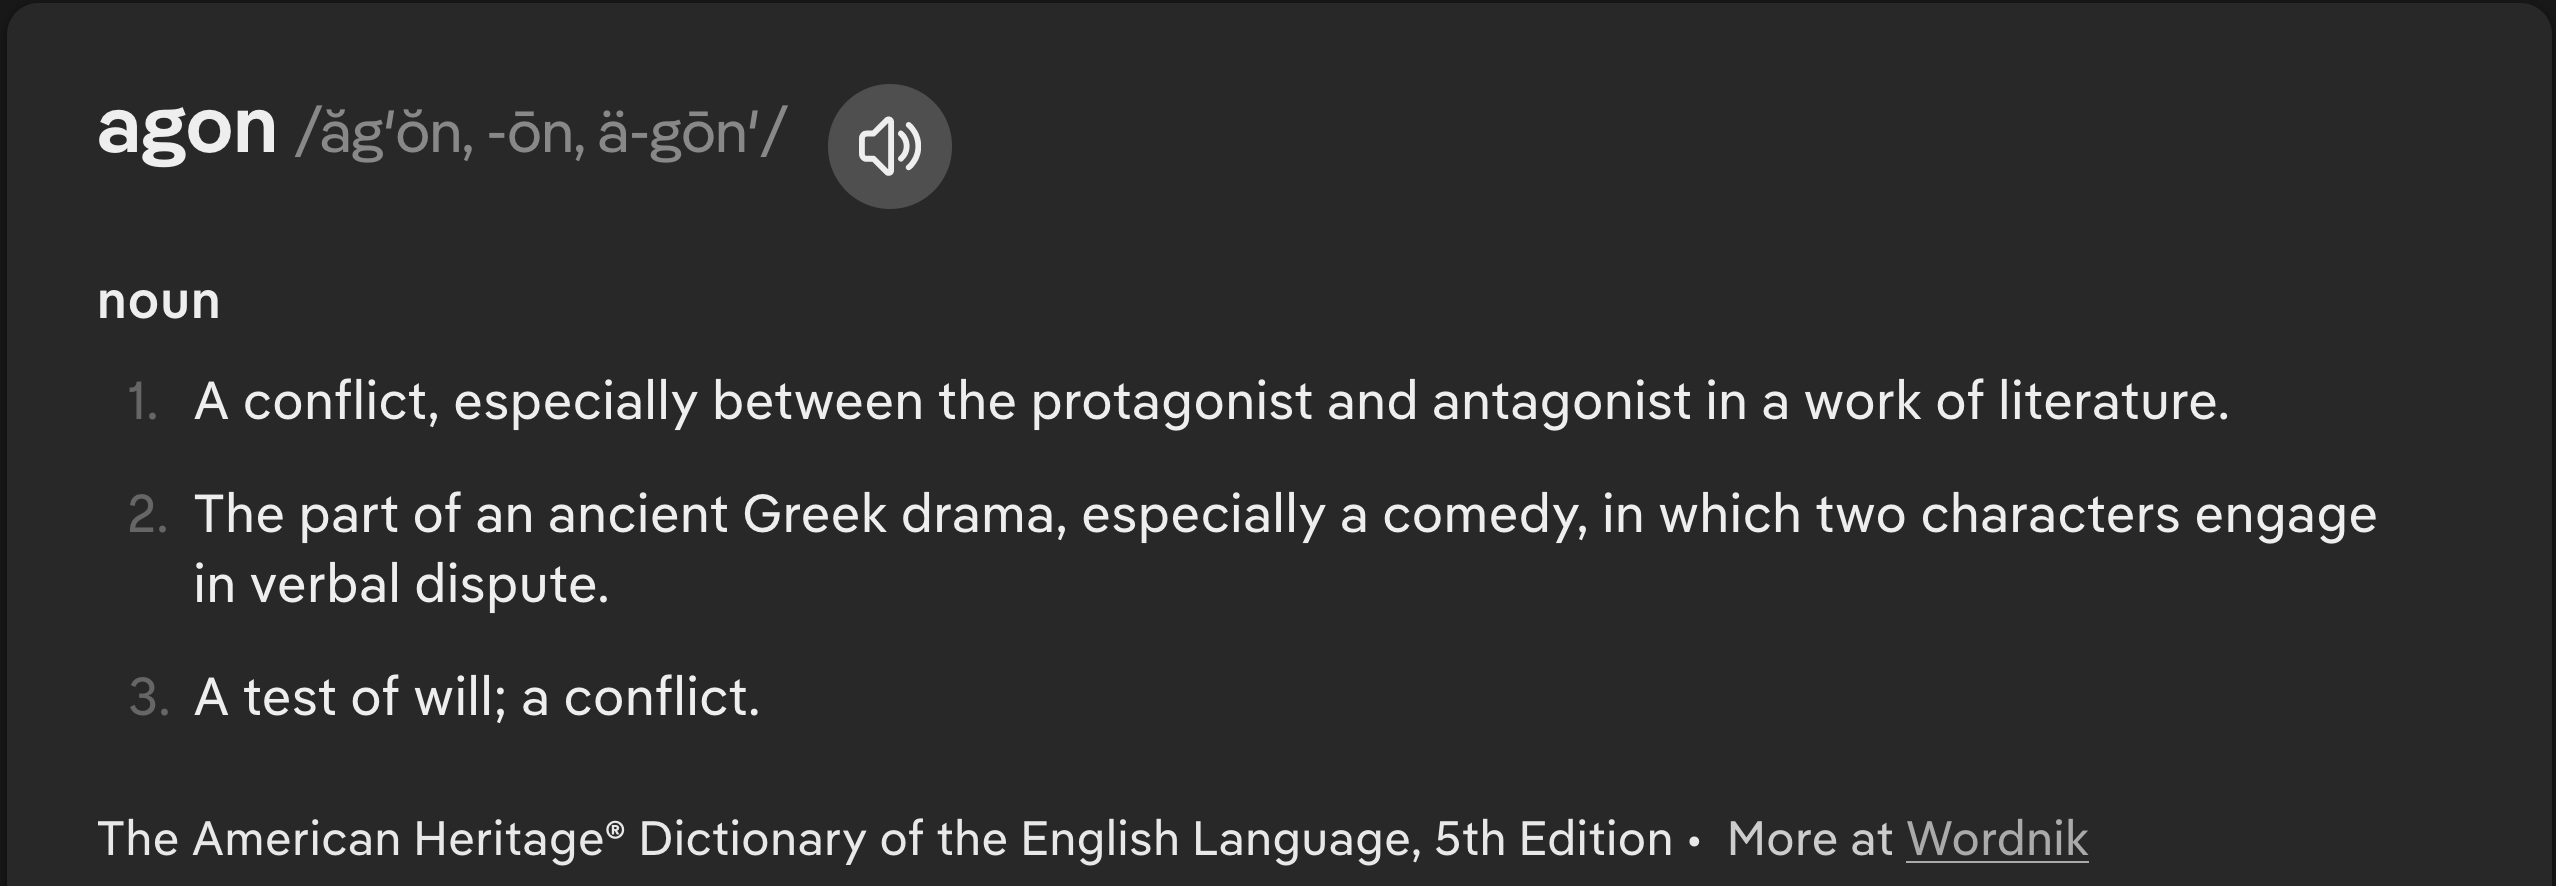
\includegraphics[width=14cm]{figures/Screenshot Agon Def.png}
\end{frame}

\begin{frame}{Overview}
    \begin{center}
        \begin{enumerate}
            \item[\faProjectDiagram] \textbf{Framework Construction and Visualisation}\\
            Interactive graph editor with automatic layouts and physics simulation
            \item[\faBalanceScale] \textbf{Semantical Reasoning}\\
            Extension- and ranking-based semantics, with enumeration and credulous / sceptical acceptance.
            \item[\faShareSquare] \textbf{Export and Sharing}\\
            Export to \LaTeX, SVG, TGF, and the ICCMA AF format, or share by URL
            \item[\faDice] \textbf{Random Generation}\\
            Random frameworks from \textcolor{WildStrawberry}{8} configurable graph generators
            \item[\faGraduationCap] \textbf{Tutorials and References}\\
            \textcolor{WildStrawberry}{10+} tutorials and a glossary with definitions and literature references
        \end{enumerate}
    \end{center}
\end{frame}

\begin{frame}{The zoo of formal argumentation, in one browser tab}
    \centering
    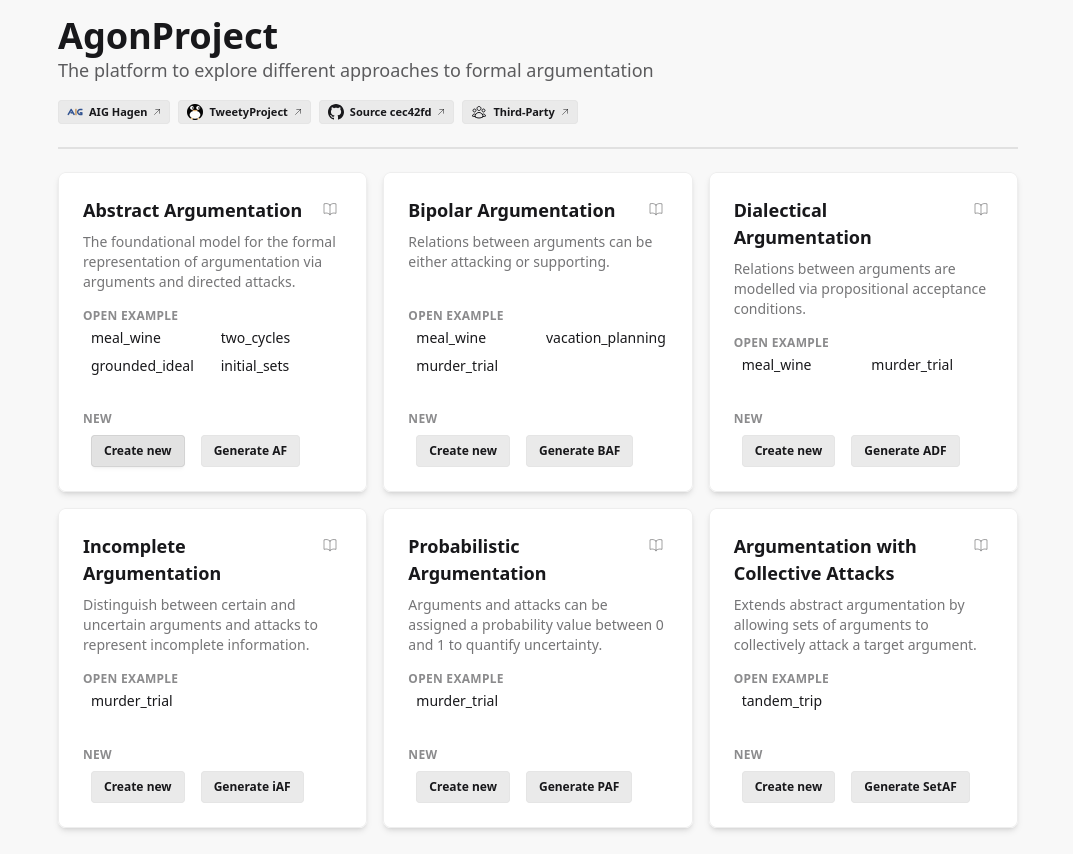
\includegraphics[width=9cm]{figures/screenshot-landing.png}
\end{frame}

\begin{frame}{Extension \& Ranking Semantics}
    \centering
    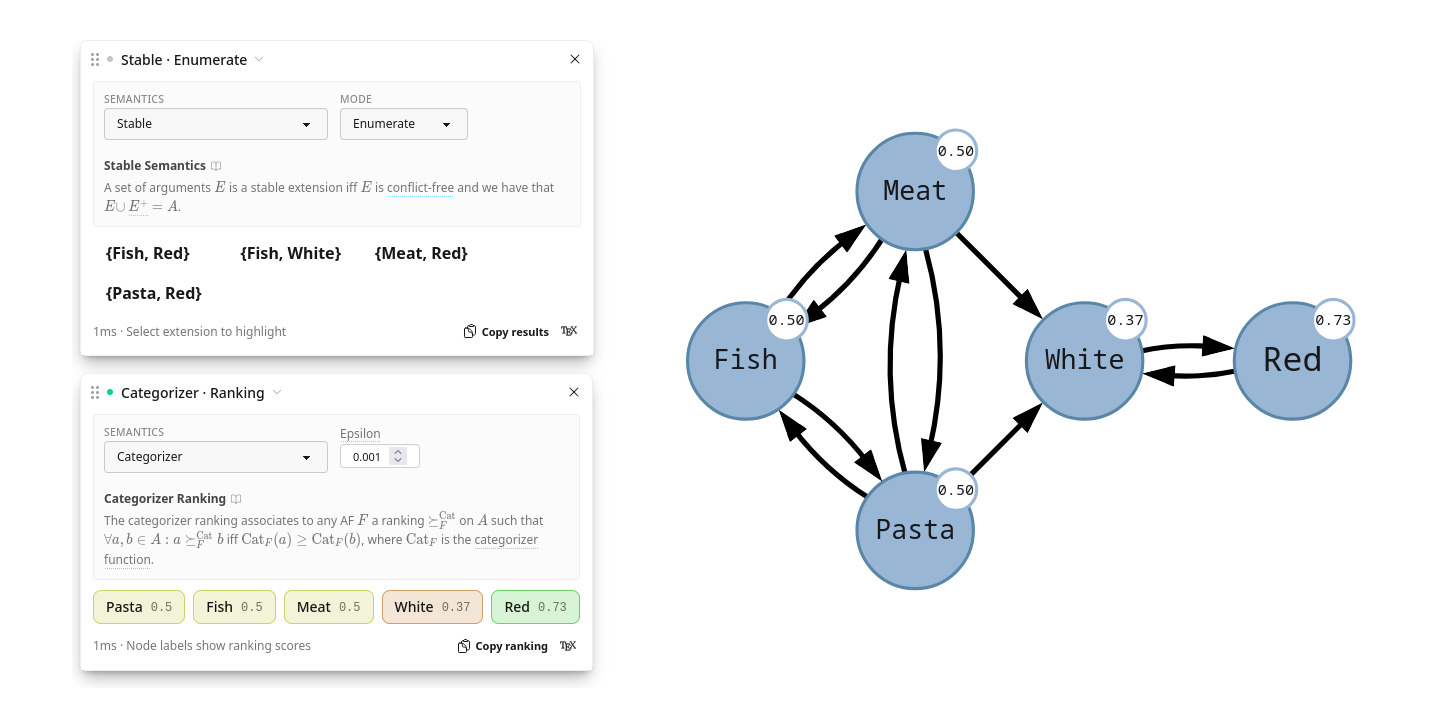
\includegraphics[width=14cm]{figures/screenshot-af.png}
\end{frame}

\begin{frame}{Supported Semantics}
    \begin{center}
        \begin{enumerate}[leftmargin=3cm]
            \item[\bf{Classical}] conflict-free, admissible, complete, grounded, preferred, stable
            \item[\bf{Admissibility-based}] ideal, semi-stable, eager, strong admissibility, initial sets, \dots
            \item[\bf{Non-admissible}] naive, CF2, SCF2, stage, stage2, (strongly) undisputed
            \item[\bf{Meta-families}] weak admissibility, (semi-)qualified, vacuous-reduct, serialisable
            \item[\bf{Argument-rankings}] burden, categoriser, counting, discussion, iterated graded defense,\\ probabilistic, propagation, serialisability, strategy-based, \dots
        \end{enumerate}
    \end{center}    
\end{frame}

\begin{frame}{ADFs \& Highlighting}
    \centering
    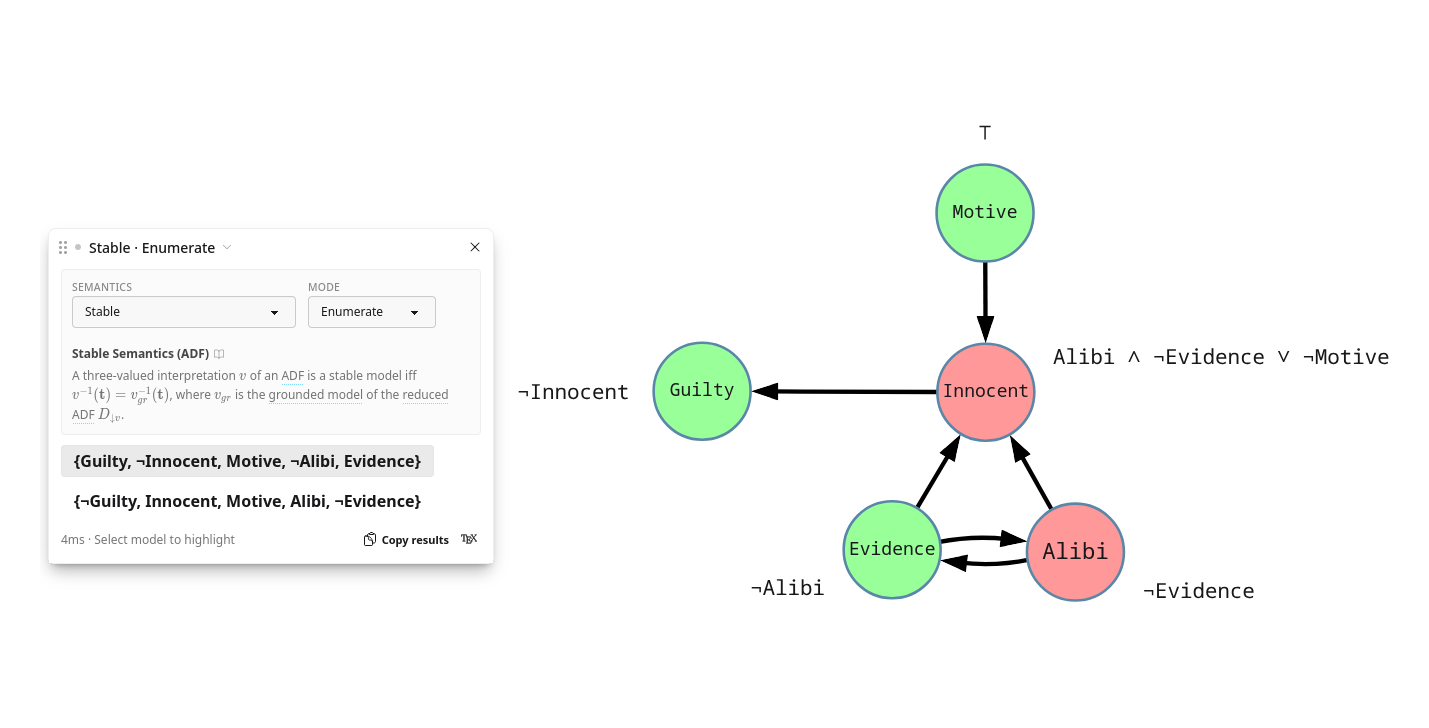
\includegraphics[width=14cm]{figures/screenshot-adf.png}
\end{frame}

\begin{frame}{Collective attacks \& Exporting}
    \centering
    
\includegraphics[width=14cm]{figures/screenshot-setaf.png}
\end{frame}

\begin{frame}{Dedicated mobile UI}
    \centering
    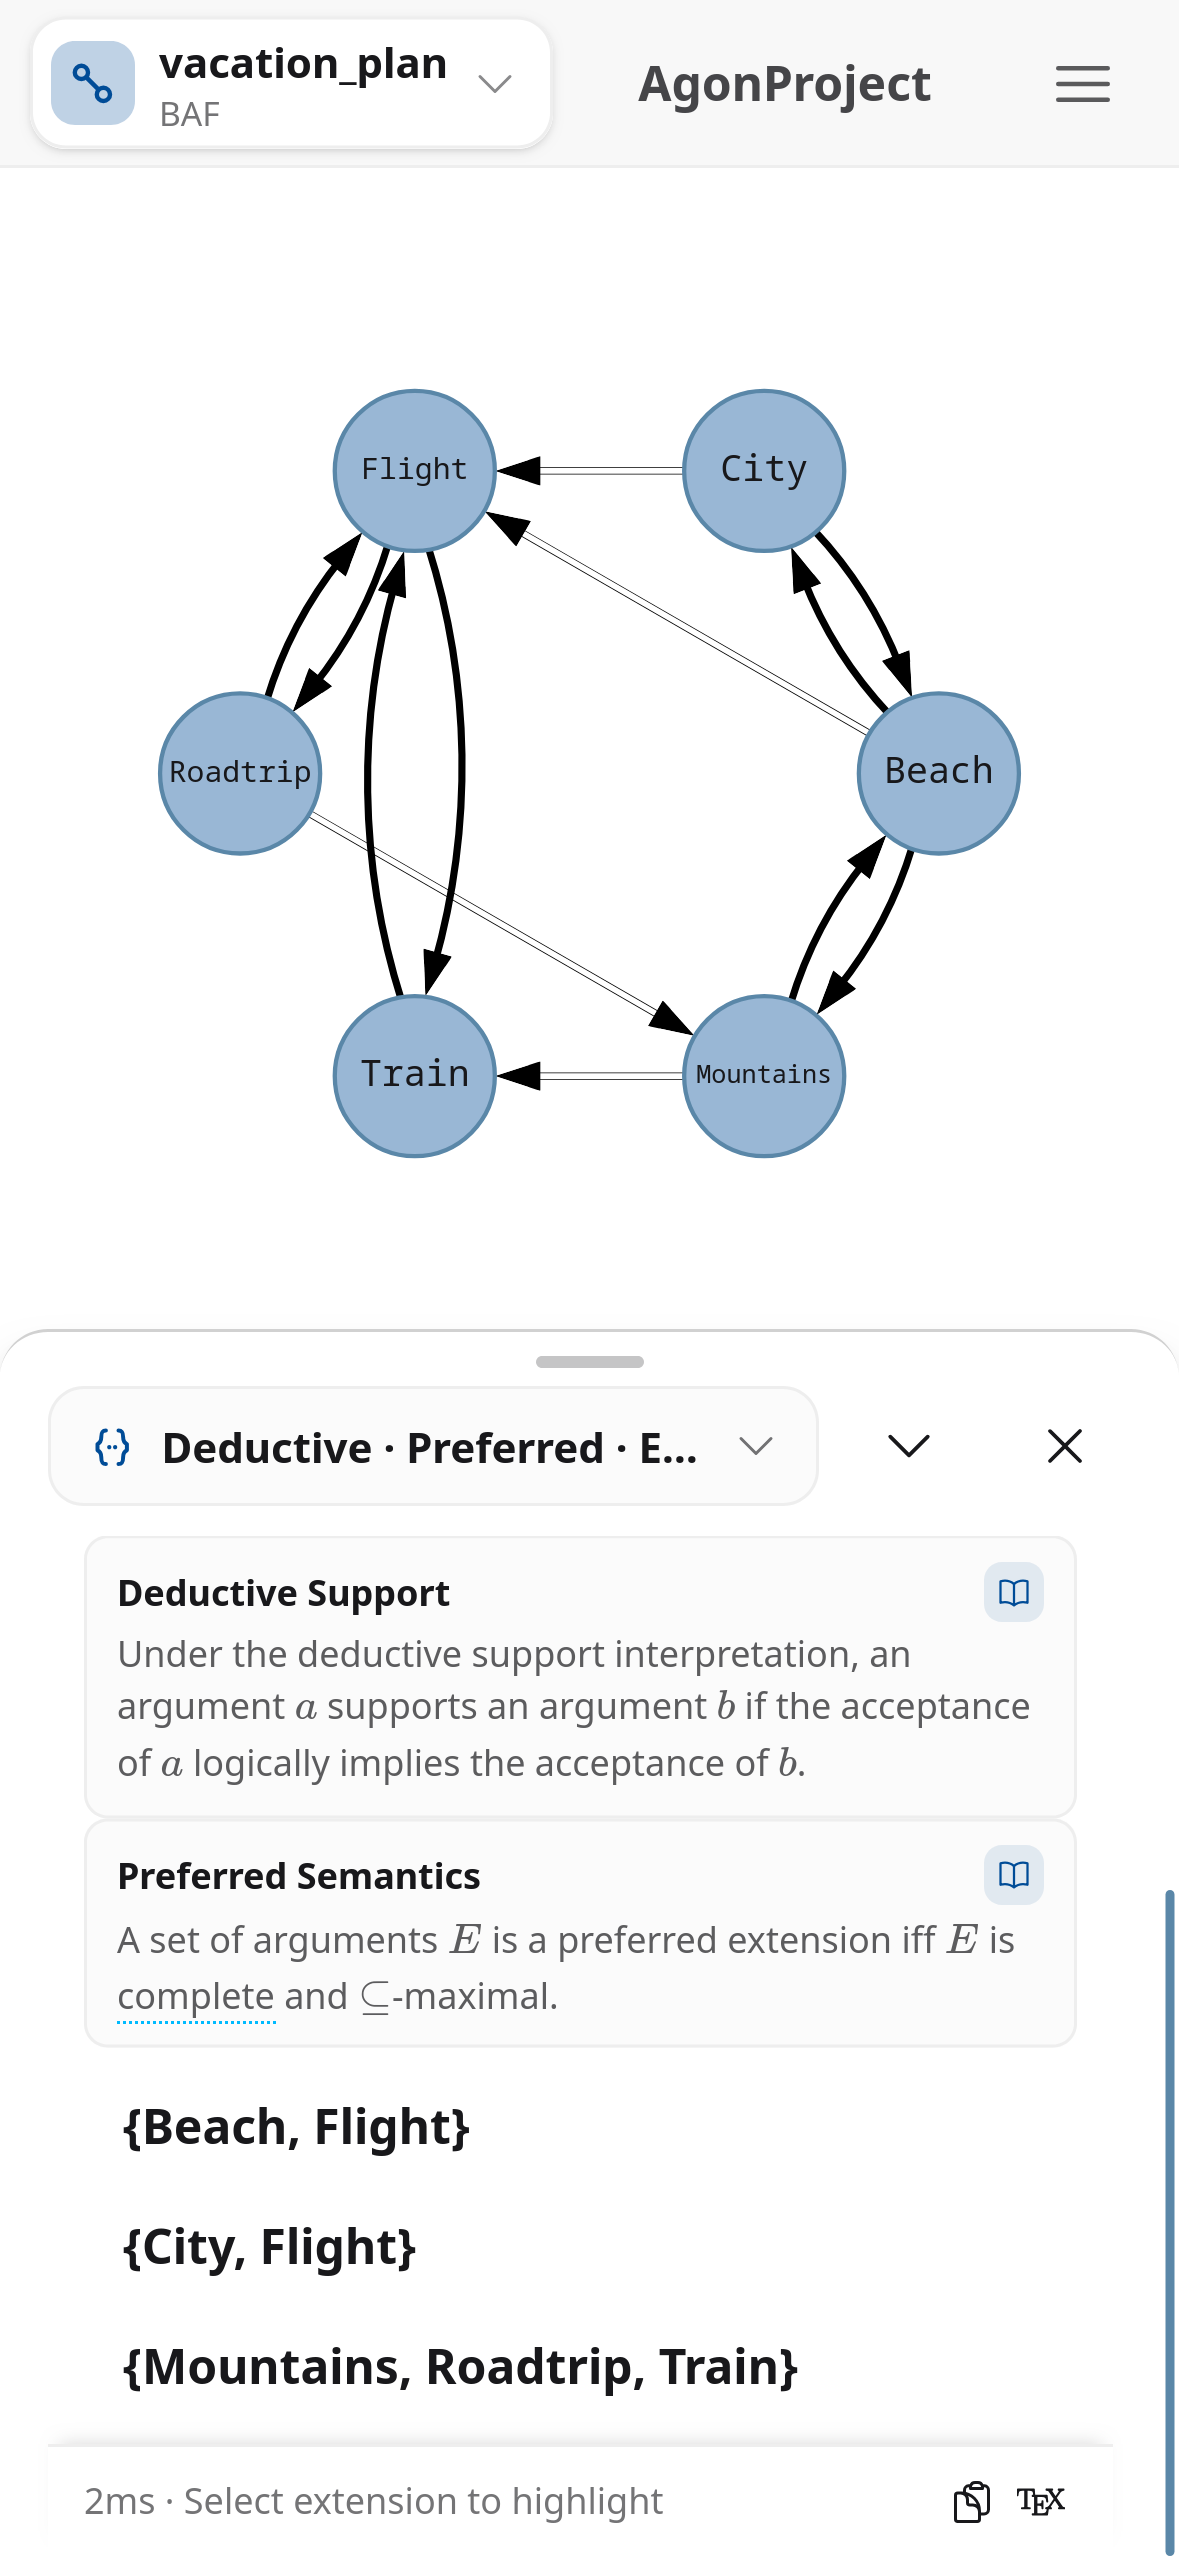
\includegraphics[width=3cm]{figures/screenshot-mobile-eval.png}
    
\includegraphics[width=3cm]{figures/screenshot-mobile-generate.png}
    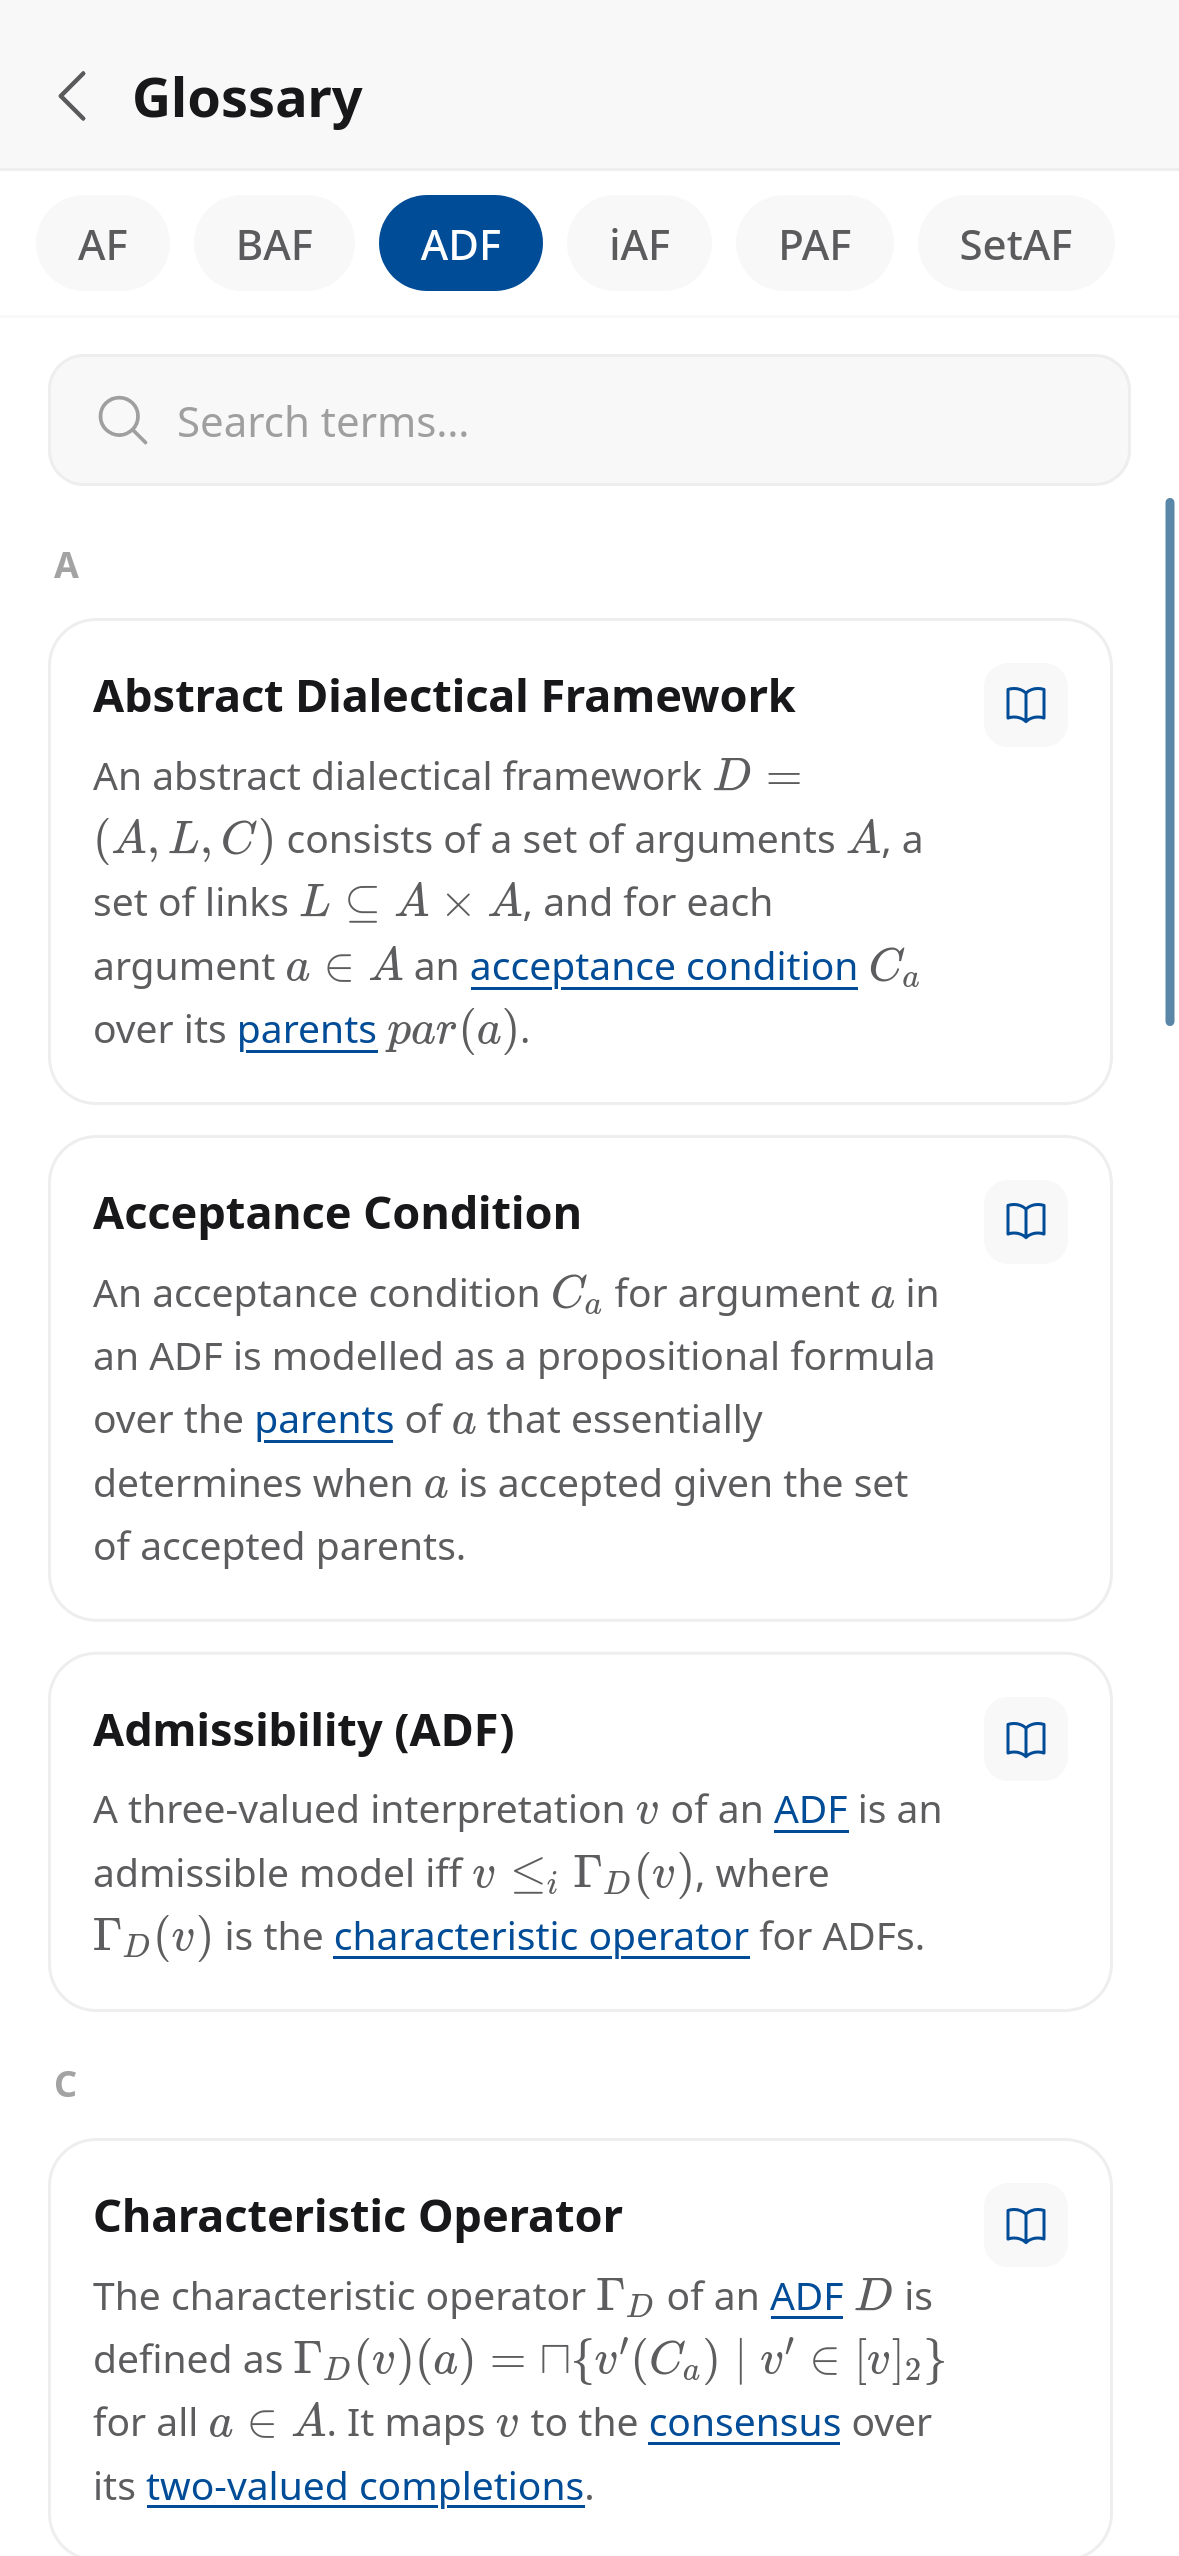
\includegraphics[width=3cm]{figures/screenshot-mobile-glossary.png}
    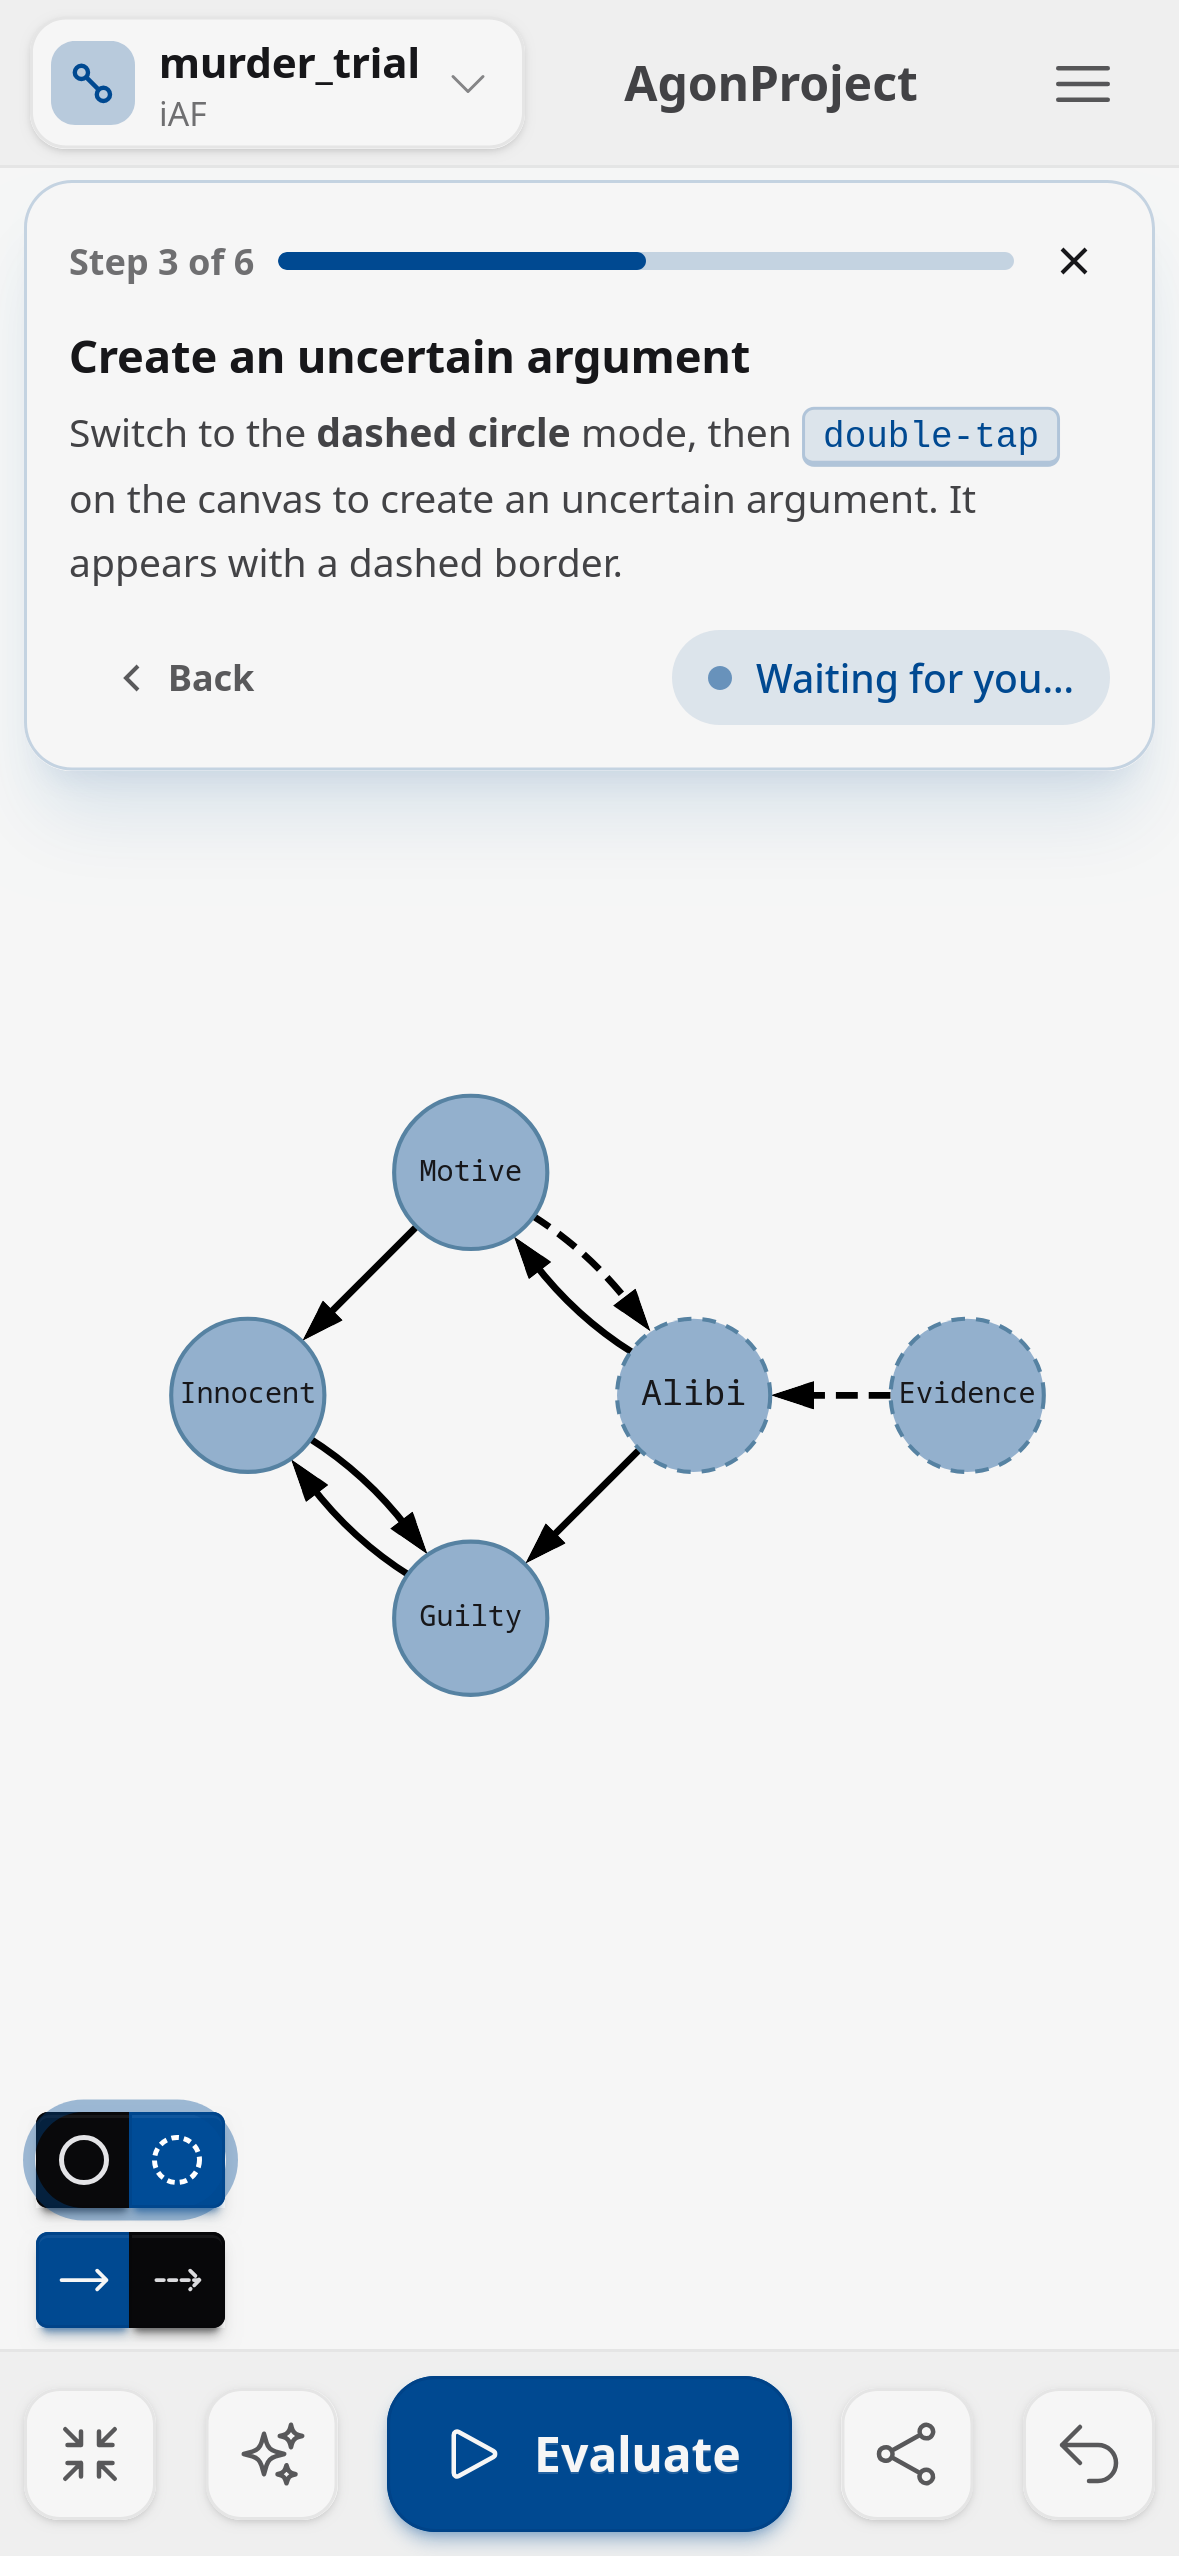
\includegraphics[width=3cm]{figures/screenshot-mobile-tutorial.png}
\end{frame}

% \begin{frame}{Scan to Try Live}
%     \begin{center}
%             \centering
%             \tikz\node[fill=white, rounded corners=7pt, inner sep=8pt]
%                 {\qrcode[height=3.4cm]{http://agon.tweetyproject.org}};
%             {\ttfamily\bfseries\fontsize{38}{46}\selectfont agon.tweetyproject.org}
%     \end{center}
% \end{frame}

\begin{frame}{Outlook}
    \begin{enumerate}
        \item[$\bullet$] more formalisms, e.g., \textbf{ABA}, \textbf{weighted AFs}, \textbf{BSAFs}, \textbf{claim-augmented AFs}
        \item[$\bullet$] benchmark generators from the ICCMA ecosystem
        \item[$\bullet$] other reasoning approaches, e.g., acceptance explanations
    \end{enumerate}
    \begin{center}
            \centering
            \tikz\node[fill=white, rounded corners=7pt, inner sep=8pt]
                {\qrcode[height=3.4cm]{http://agon.tweetyproject.org}};
            {\ttfamily\bfseries\fontsize{30x}{46}\selectfont agon.tweetyproject.org}
    \end{center}
\end{frame}

\appendix

% \section{Appendix}

% \begin{frame}{Appendix}
%     This is an appendix.
%     \begin{itemize}
%         \item Page numbers start from the beginning.
%     \end{itemize}
% \end{frame}

\end{document}
